% コンパイル方法: lualatex filename.tex
\RequirePackage{plautopatch}

\documentclass[a4paper, 10pt]{ltjsarticle}


% マージン設定
\usepackage[top=20mm, bottom=20mm, left=20mm, right=20mm]{geometry}

% LuaLaTeX用日本語対応パッケージ
\usepackage{luatexja}
\usepackage{luatexja-fontspec}

% 必要なパッケージ
\usepackage{fontspec}
\usepackage{titlesec}
\usepackage{graphicx}
\usepackage{amsmath}
\usepackage{amssymb}
\usepackage{hyperref}
\usepackage[english, japanese]{babel}
\usepackage{multicol} % 二段組用パッケージ
\usepackage{indentfirst}
\usepackage{tikz} % カスタム点線用
\usepackage{authblk} % 著者・所属パッケージ
\usepackage{here}
\usepackage{caption}
\usepackage{tabularx}

% \setmainfont[Ligatures=TeX]{Times New Roman}
% \setmainjfont[BoldFont=MS Gothic]{MS Mincho}

\renewcommand{\baselinestretch}{0.95}

% セクション見出しのカスタマイズ
\titleformat{\section}
  {\fontsize{10pt}{10pt}}
  {\thesection.}
  {1em}{}

\titleformat{\subsection}
  {\fontsize{10pt}{10pt}}
  {\thesubsection}
  {1em}{}

\titleformat{\subsubsection}
  {\fontsize{10pt}{10pt}}
  {\thesubsubsection}
  {1em}{}

  \setlength{\parindent}{1em}

\captionsetup[table]{skip=0pt}
% \setlength{\belowcaptionskip}{1em} % キャプション下の余白を設定



\titlespacing*{\section}{0em}{1em}{0em}
\titlespacing*{\subsection}{0em}{1em}{0em}

\pagestyle{empty}


\begin{document}

% \setlength{\abovedisplayskip}{1em}
% \setlength{\belowdisplayskip}{1em}
\setlength{\columnsep}{7.5mm}

\twocolumn[
    \begin{center}
        {\vspace{-1em}}

        {\fontsize{15pt}{15pt}\selectfont{クロスレイヤシミュレータにおける無線LAN評価モデルの検討}}

        {\vspace{1.3em}}

        {\fontsize{13pt}{13pt}\selectfont{A Study of a Wireless LAN Evaluation Model in a Cross-Layer Simulator}}
    \end{center}

    \vspace{0.1em}

    \begin{flushright}
      {\fontsize{11pt}{11pt}\selectfont{T5-16 \, 下沢亮太郎}}
      \\
      {\fontsize{11pt}{11pt}\selectfont{指導教員 \, 設樂勇}}
    \end{flushright}

    \vspace{1em}

    \thispagestyle{empty}
]

\section{緒言}
近年,無線通信端末利用者の急増に伴い様々な場所で無線通信システムが利用されており,今後も利用の増加と発展が見込まれている.近年の無線通信技術の進歩に伴い,システムが高機能化・複雑化しており,従来のようにレイヤごとに独立した性能評価を行う手法では通信全体の実用的な評価を十分に行うことが困難になりつつある.

そのため,通信全体をクロスレイヤで評価できる計算機シミュレータの開発が求められている.本研究ではクロスレイヤシミュレータにおけるMACレイヤの挙動をシミュレートする機能を開発を行い,その有効性を評価した.


\section{無線LAN通信の特性}
\subsection{CSMA/CA(Carrier Sense Multiple Access with Collision Avoidance)}
無線LANの規格であるIEEE 802.11では,CSMA/CAと呼ばれる方式が採用されている.この方式は,送信前にチャネルが空いているかどうかを確認し,空いている場合に送信を行う方式である.図\ref{CSMA/CA}にCSMA/CAの概要を示す.

CSMA/CAでは,端末は送信チャネルをキャリア感知(Carrier Sense)し,チャネルが空いているタイミングでパケット送信を試みる.もしチャネルが使用中であれば,一定時間バックオフを行う.このとき,各端末はランダムに生成したスロット数に従い待機し,他の端末との衝突を回避する.



\begin{figure}[H]
  \centering
  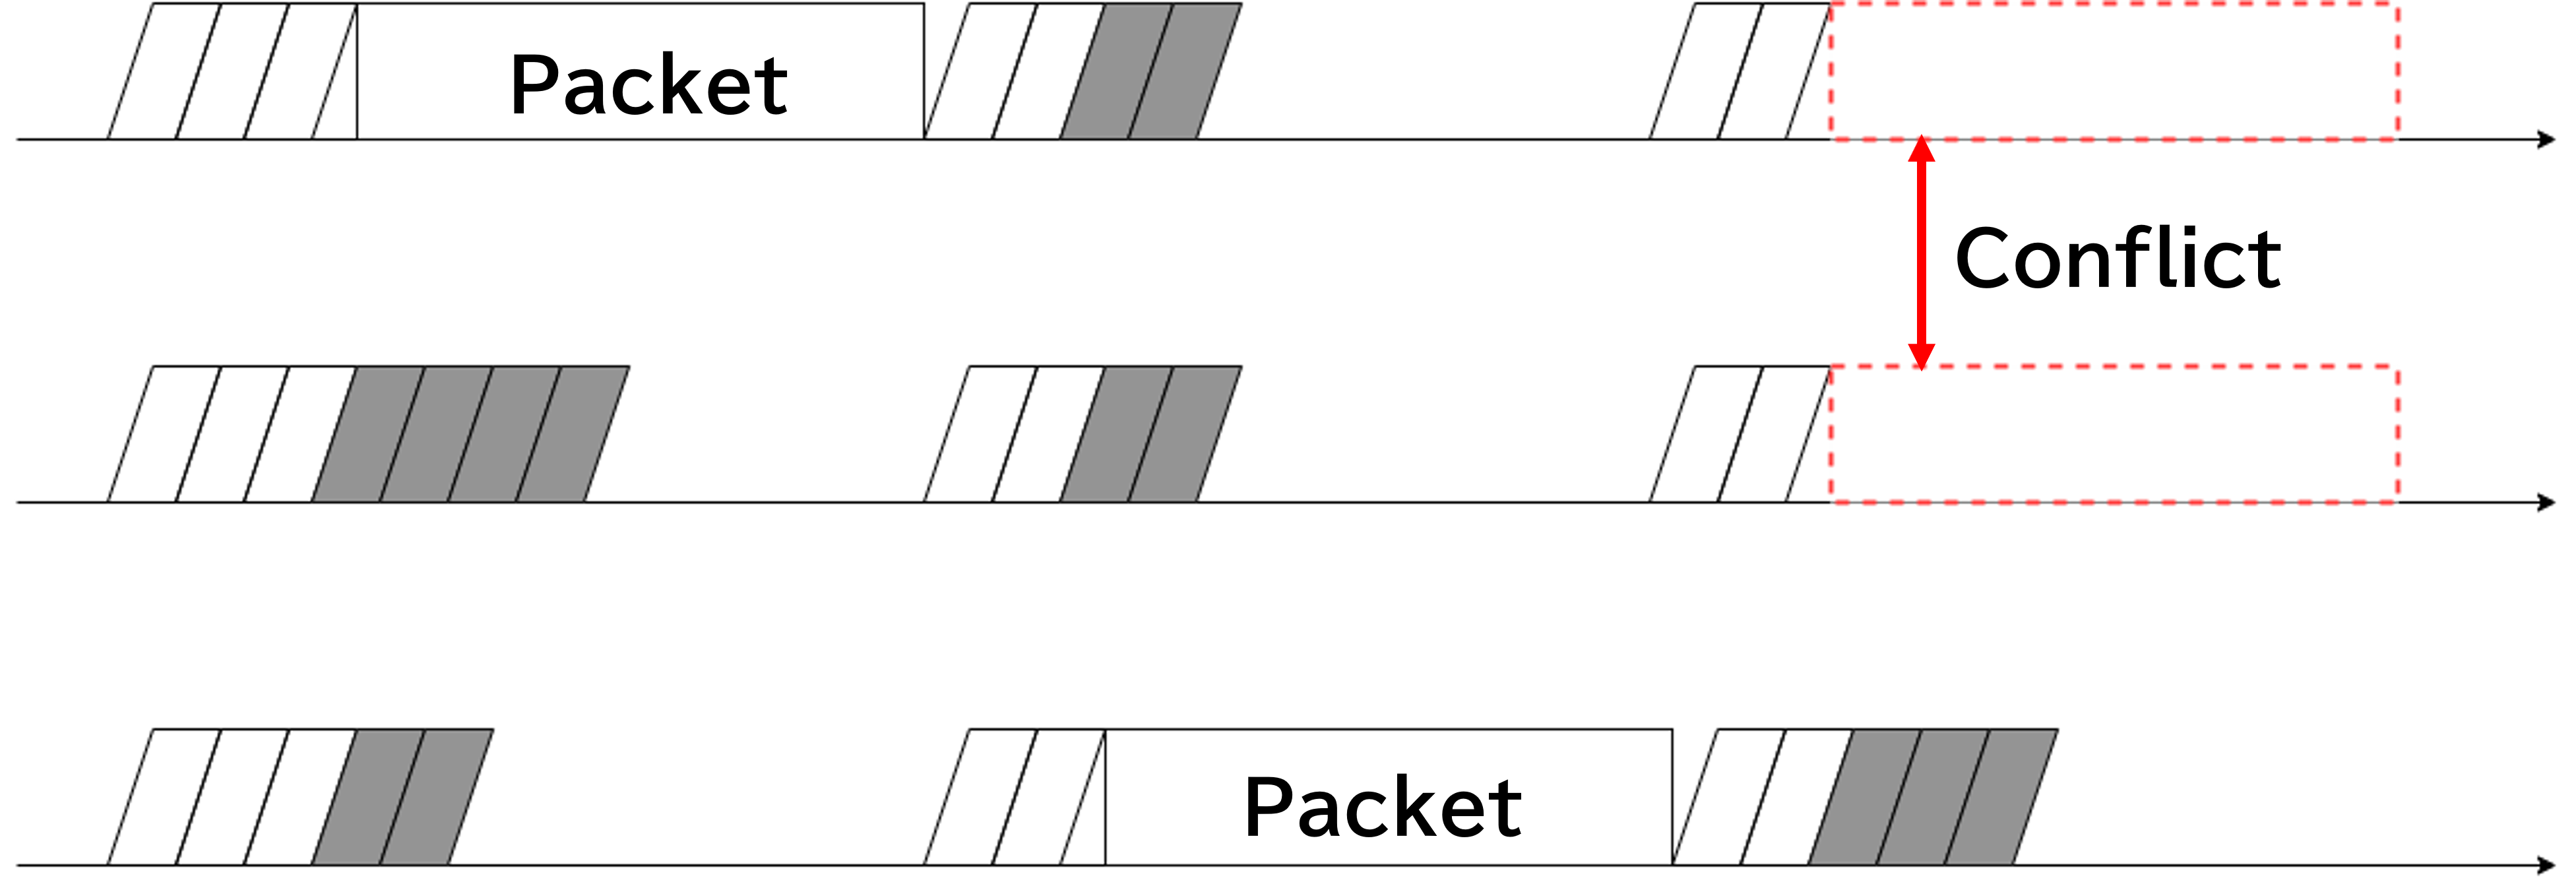
\includegraphics[width=1\columnwidth]{./assets/csmaca-1.png}
  \caption{CSMA/CA概要}
  \label{CSMA/CA}
\end{figure}

\subsubsection{CW(Contention Window)}
バックオフ時に用いるコンテンションウィンドウは,衝突回数や再送制御のパラメータに応じて変化する.再送回数を$n$とするとCWの最大値は


% 再送回数を$n$とするとCWの最大値は

\begin{align}
  \text{cw\_max} &= 2^{4 + n} - 1
\end{align}

となり,スロット数$s$は

\begin{align}
  s &= \mathrm{randint}(1, \, \min(\text{cw\_max}, \, 1023))
  \label{slot}
\end{align}

% \begin{align}
%   \text{slots} &= \mathrm{randint}(1, \, \min(\text{cw\_max}, \, 1023))
% \end{align}


で定義される.

本研究では,上記の式を用いて,各端末が送信を試みる際の待機時間を動的に変化させる処理を実装した.

CSMA/CAによるランダムアクセスは,多数の端末が同時にアクセスしようとする場合でも,一部の端末が優先的にチャネルを占有する状況を回避できる利点を持つ.そのため,大規模な無線LAN環境下での通信効率を左右する重要な仕組みとして知られている.


\subsection{パケット構成モデル化}

UDPレベルでの無線LAN通信をシミュレートするために,簡易的にパケットを構成するモデルを作成した.図\ref{packet}に,モデル化されたパケットの構成図を示す.

\begin{figure}[H]
  \centering
  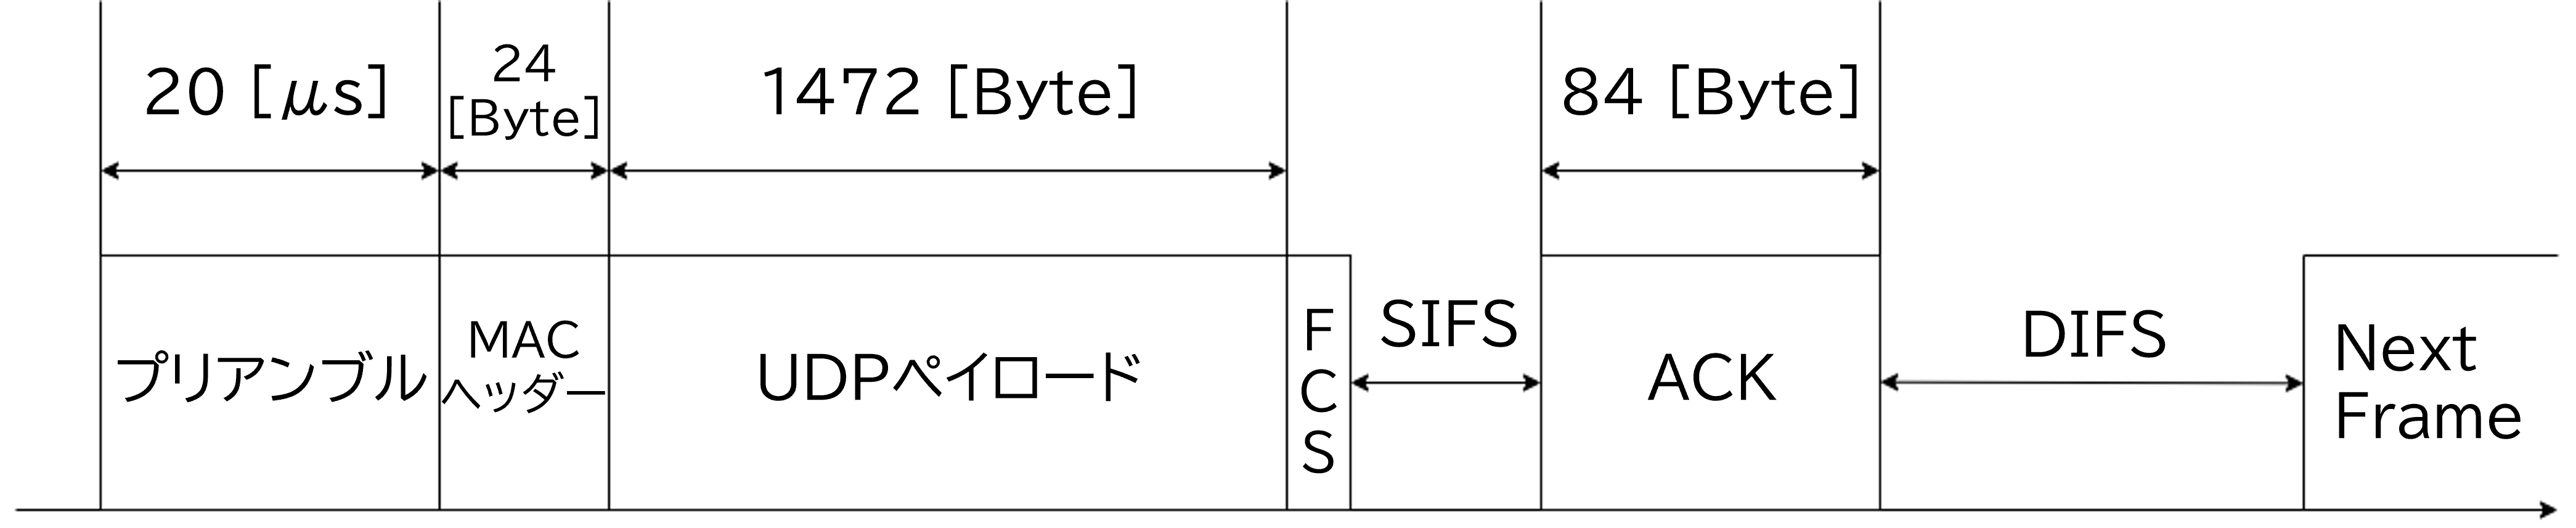
\includegraphics[width=1\columnwidth]{./assets/packet.png}
  \caption{モデル化されたパケット構成図}
  \label{packet}
\end{figure}


% \section{提案手法}
% \subsection{User class}

\section{実装とシミュレーション設定}
\subsection{Userクラスの設計}
本研究のシミュレータ実装では、各端末を\texttt{User}クラスとして定義し、端末ごとのCWや再送回数などを管理している.表\ref{tab:user-class}に主なメンバ変数と役割をまとめる.

\begin{table}[H]
  \centering
  \caption{Userクラスのメンバ変数とメソッドの一覧}
  \label{tab:user-class}
  \begin{tabularx}{\columnwidth}{lX}
    \hline
    % \textbf{名称} & \textbf{説明} \\
    名称 & 説明 \\
    \hline
    \multicolumn{2}{l}{メンバ変数} \\
    \hline
    \texttt{id} & 端末を識別するためのID\\
    \texttt{num\_re\_trans} & 再送回数\\
    \texttt{slots} & スロット数\\
    \texttt{num\_transmitted} & 送信成功回数\\
    \texttt{data\_transmitted} & 送信したデータ量 \, [bit]\\
    \hline
    \multicolumn{2}{l}{主なメソッド} \\
    \hline
    \texttt{calc\_slots()} &(\ref{slot})式に従い\texttt{slots}を決定\\
    \texttt{re\_transmit()} & 再送処理\\
    \texttt{reset\_slots()} & 新たに\texttt{slots}を割り当てる\\
    \hline
  \end{tabularx}
\end{table}

\subsection{シミュレーションパラメータ}
表\ref{tab:sim-param}に、本研究で用いた代表的なシミュレーションパラメータを示す。バージョン違い(IEEE 802.11a/b/g)によりスロット時間やDIFS/SIFSなどのタイミングパラメータが異なるため、対応するモードを選択することで、実環境に近い動作を切り替えられる。  

\begin{table}[H]
  \centering
  \caption{シミュレーションパラメータの例}
  \label{tab:sim-param}
  \begin{tabularx}{0.9\columnwidth}{@{\hspace{1em}}l@{\hspace{4.5em}}l}
    \hline
    パラメータ & 値・例 \\
    \hline
    シミュレーション時間 & 60 \, [$\mathrm{s}$] \\
    スロット時間 (802.11a) & \, 9 \, [$\mathrm{\mu s}$] \\
    DIFS (802.11a) & 34 \, [$\mathrm{\mu s}$] \\
    SIFS (802.11a) & 16 \, [$\mathrm{\mu s}$] \\
    データレート & 24 \, [Mbps] \\
    \hline
  \end{tabularx}
\end{table}


\section{結果, 考察}
図\ref{fig:simulation-result}に,横軸を端末数,縦軸をスループットとし,シミュレーション結果と理論値を併せてプロットしたグラフを示す.
% 横軸に端末数,縦軸にスループットを取ったグラフを図\ref{fig:simulation-result}に示す.

端末数がが増加するにつれて理論値との差が大きくなるが,それは参考にした論文\cite{paper}とのモデル化した時の差によるものだと考える.

\begin{figure}[H]
  \centering
  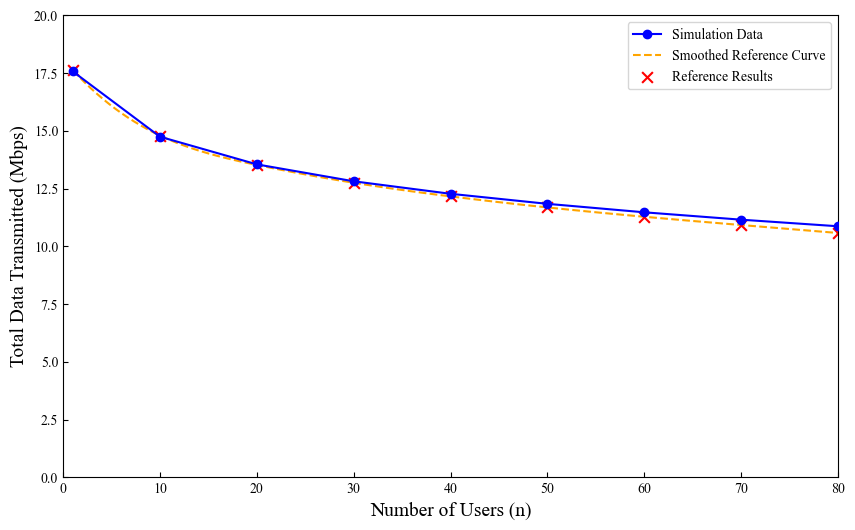
\includegraphics[width=1\columnwidth]{./assets/g3.png}
  \caption{シミュレーション結果}
  \label{fig:simulation-result}
\end{figure}


\section{結言}
本研究では,クロスレイヤシミュレータの一部である無線LANシミュレータを開発し,CSMA/CAを中心とした動作のモデル化と検証を行った.

現在の方法では通信が連続して行われているが,ポアソン分布に従った時間だけ離すことで実際の通信頻度に近い状況を再現することや,各ステーションに距離の概念を持たせて自由空間伝搬による減衰を考慮することが今後の課題である.

\begin{thebibliography}{9}
  \bibitem{midori}守倉正博, 久保田周治, 『インプレス標準教科書シリーズ 改訂三版802.11 高速無線LAN教科書』, 株式会社インプレスコミュニケーションズ, 2016年
  \bibitem{paper}Y. Morino, T. Hiraguri, H. Yoshino, K. Nishimori, T. Matsuda, ``A Novel Collision Avoidance Scheme Using Optimized Contention Window in Dense Wireless LAN Environments*'' \, \textit{IEICE TRANS. COMMUN.}, VOL.E99-B, NO.11 NOVEMBER 2016
\end{thebibliography}



\end{document}
